%
\hsection{Installing LibreOffice under Ubuntu Linux}%
\FloatBarrier%
%
\begin{figure}%
\centering%
%
\subfloat[][%
Open a \pgls{terminal} via with \ubuntuTerminal, then type \bashil{libreoffice --version} and hit~\keys{\return}. %
On my system, \libreoffice~24.2.7.2 is installed.%
\label{fig:installingLibreOfficeUbuntu1checkVersion}%
]{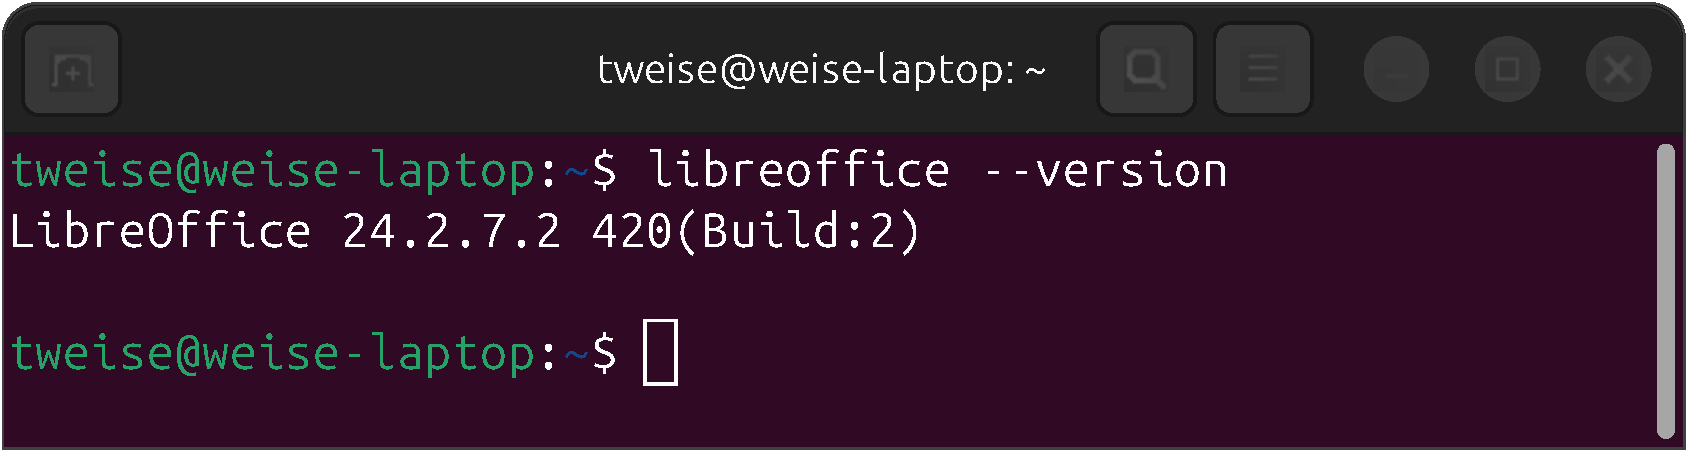
\includegraphics[width=0.7\linewidth]{\currentDir/installingLibreOfficeUbuntu1checkVersion}}%
%
\floatRowSep%
%
\subfloat[][%
We can start \libreofficeBase\ from the \pgls{terminal} by typing \bashil{libreoffice --base} and hitting~\keys{\return}.%
\label{fig:installingLibreOfficeUbuntu2runFromTerminal}%
]{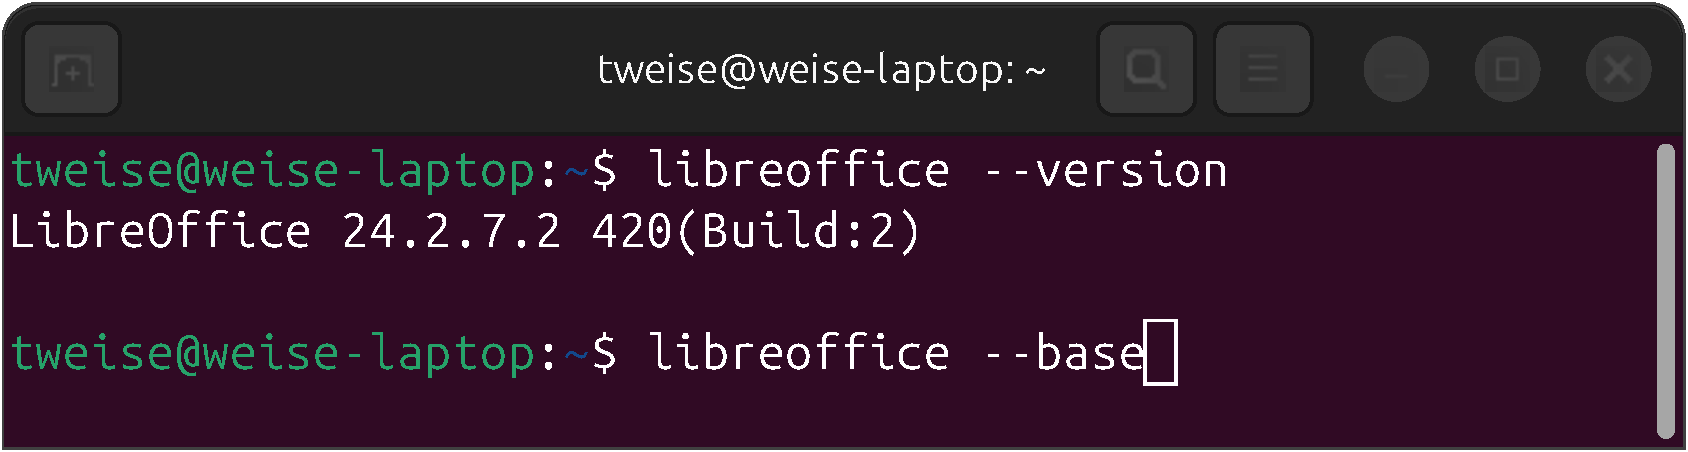
\includegraphics[width=0.7\linewidth]{\currentDir/installingLibreOfficeUbuntu2runFromTerminal}}%
%
\floatRowSep%
%
\subfloat[][%
Or we can open the dash by hitting~\keys{\OSwin}, type \textil{libreoffice}, and then clicking on the symbol for \libreofficeBase.%
\label{fig:installingLibreOfficeUbuntu4runFromDash}%
]{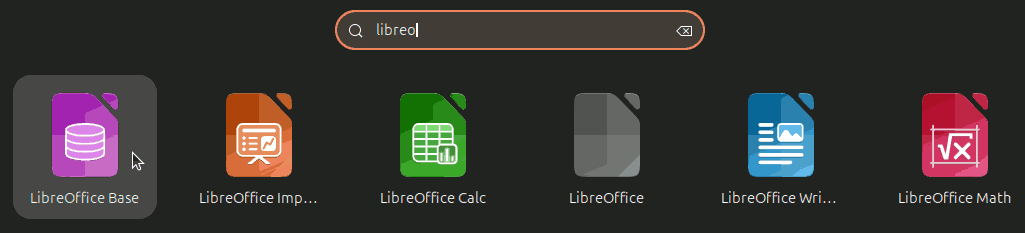
\includegraphics[width=0.65\linewidth]{\currentDir/installingLibreOfficeUbuntu4runFromDash}}%
%
\floatSep%
%
\subfloat[][%
We can also open the dash by clicking on the little \ubuntu\ symbol at the bottom-left corner of the screen.%
\label{fig:installingLibreOfficeUbuntu3openDash}%
]{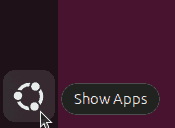
\includegraphics[width=0.33\linewidth]{\currentDir/installingLibreOfficeUbuntu3openDash}}%
%
\caption{Starting \libreofficeBase\ under \ubuntu\ if it is already installed.}%
\label{fig:installingLibreOfficeUbuntuA}%
\end{figure}%
%
\begin{figure}%
\ContinuedFloat%
\centering%
%
\subfloat[][%
The startup screen appears.%
\label{fig:installingLibreOfficeUbuntu5startupScreen}%
]{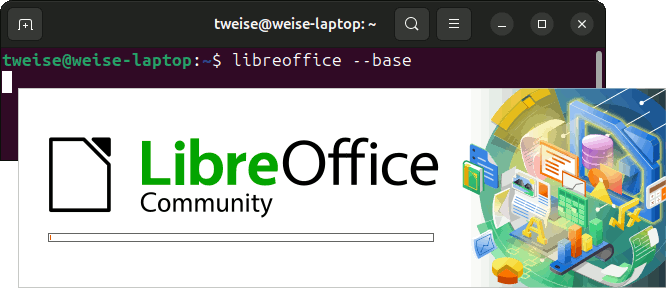
\includegraphics[width=0.8\linewidth]{\currentDir/installingLibreOfficeUbuntu5startupScreen}}%
%
\floatRowSep%
%
\subfloat[][%
The initial form of \libreofficeBase\ appears. %
We are done for now and close the program.%
\label{fig:installingLibreOfficeUbuntu6startupForm}%
]{\tightbox{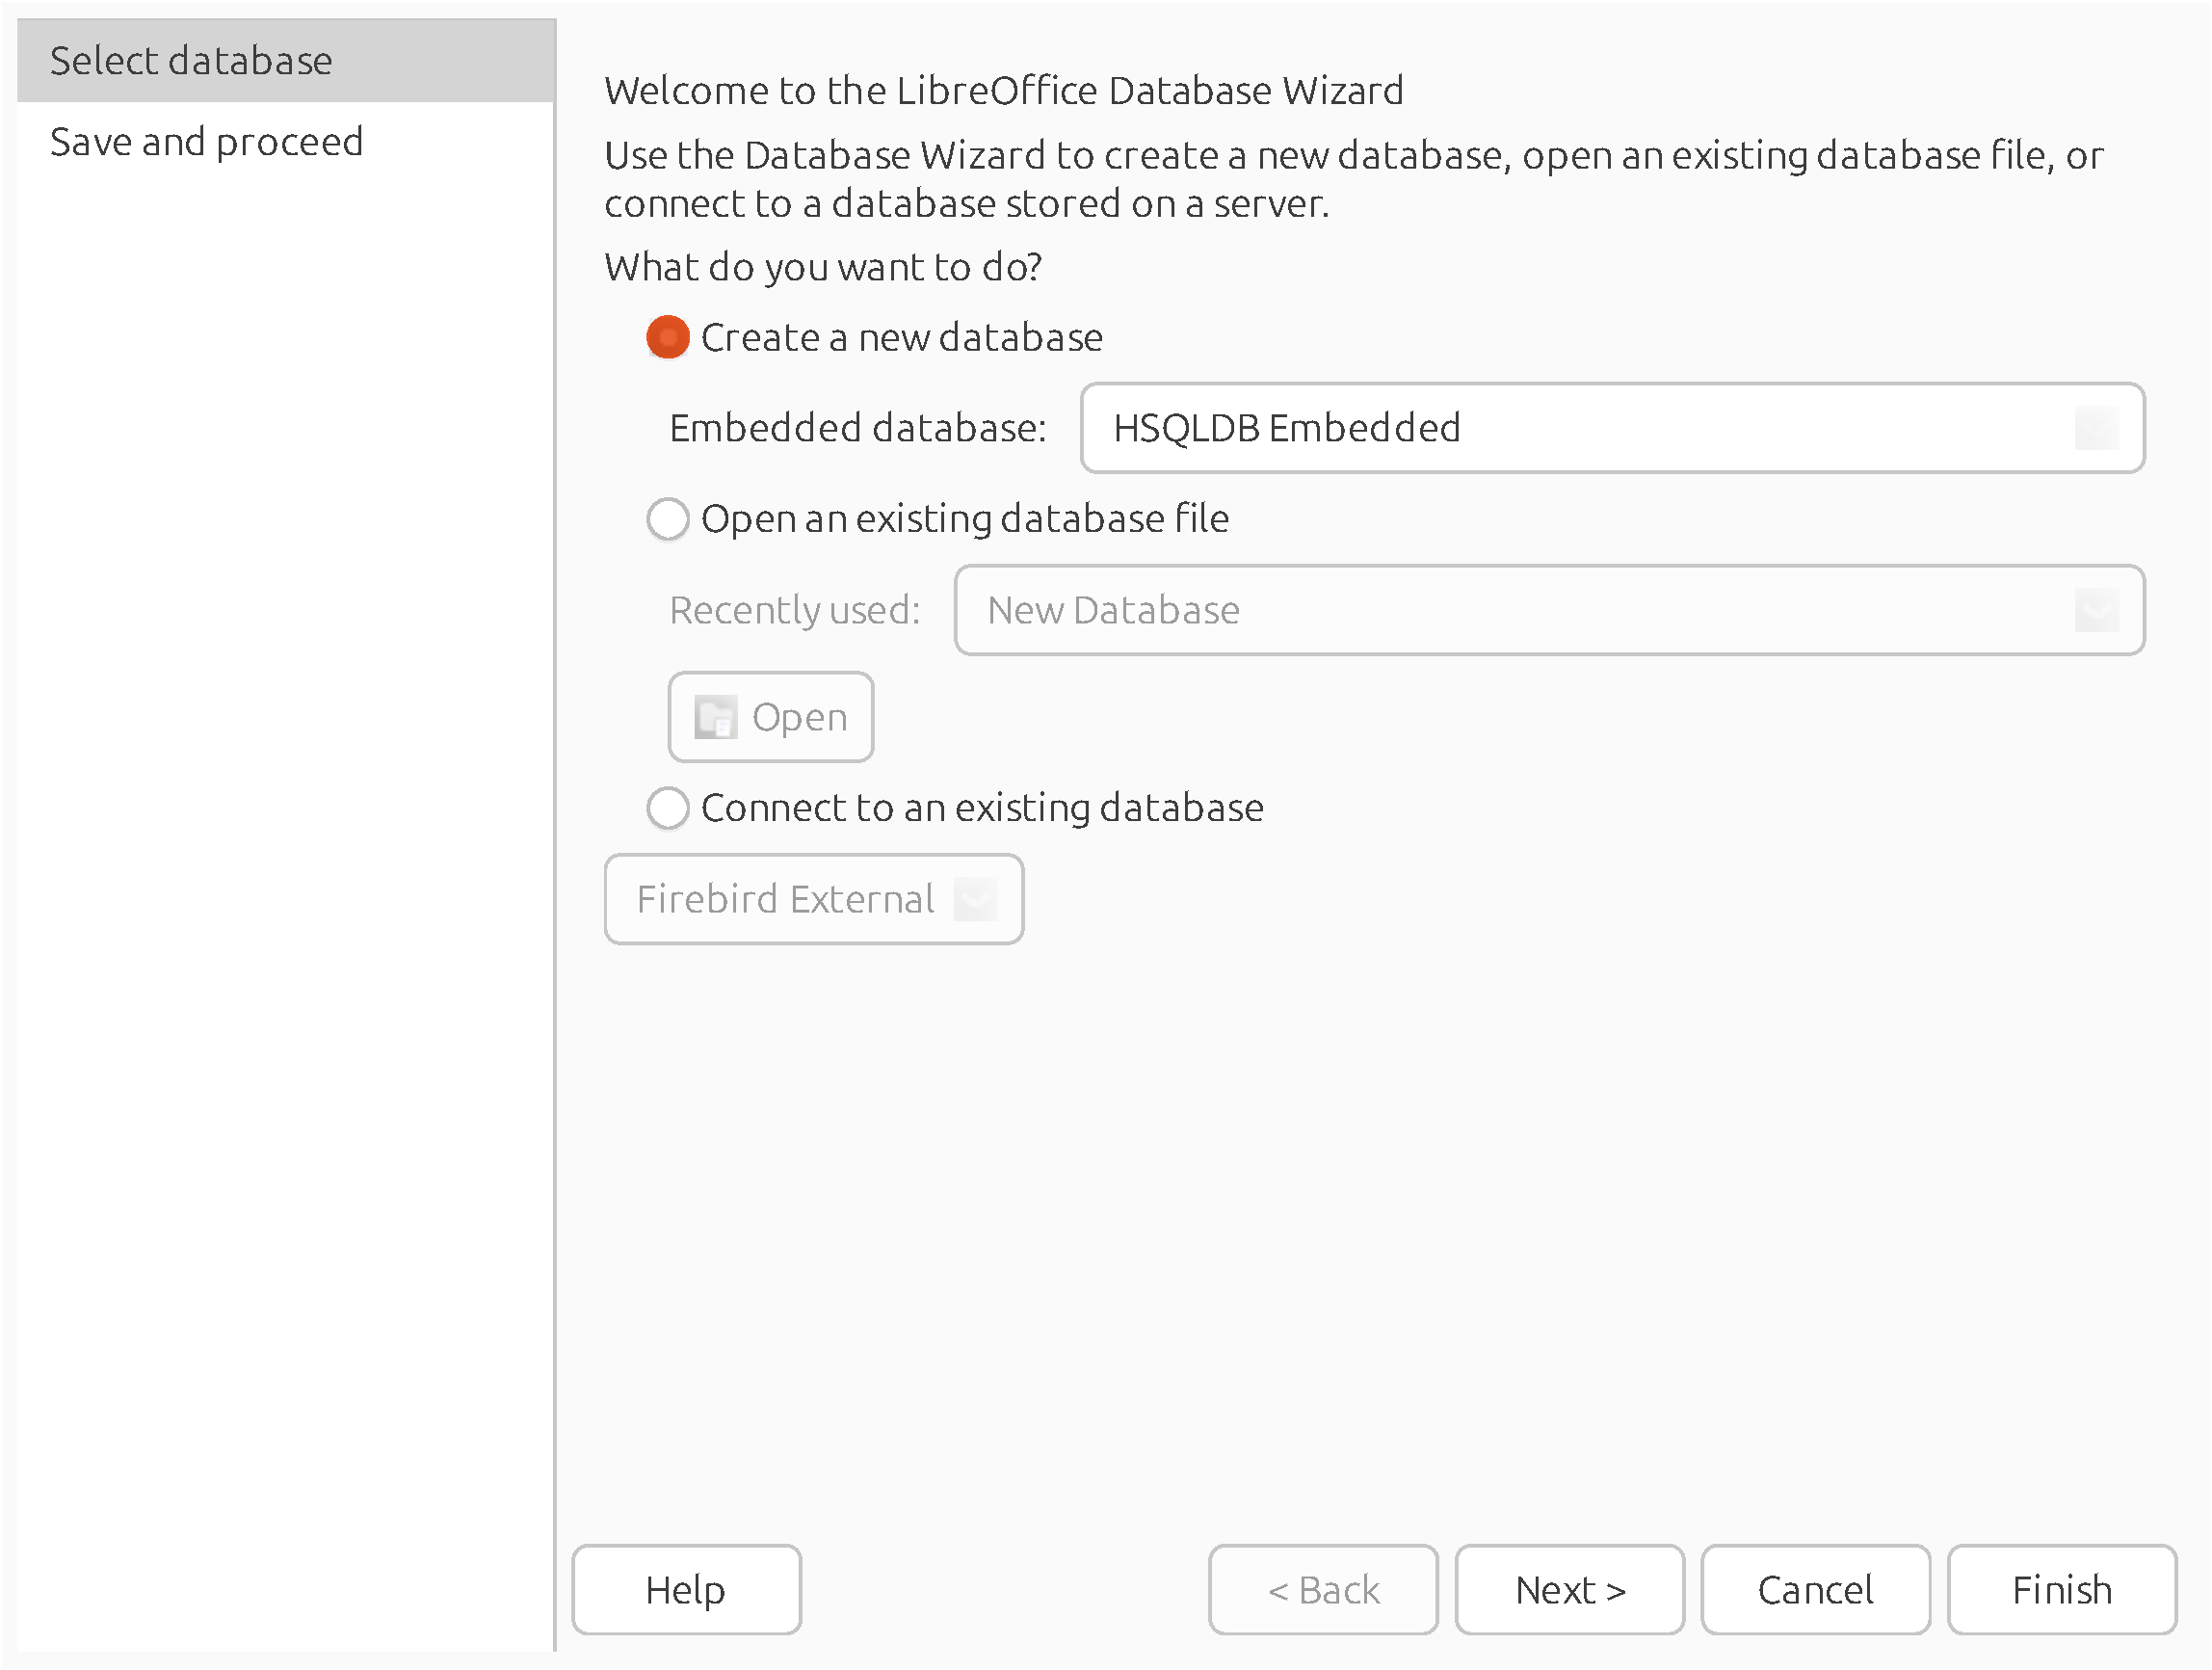
\includegraphics[width=0.8\linewidth]{\currentDir/installingLibreOfficeUbuntu6startupForm}}}%
%
\caption{Starting \libreofficeBase\ under \ubuntu\ if it is already installed.}%
\label{fig:installingLibreOfficeUbuntuB}%
\end{figure}%
%
\begin{figure}%
\centering%
%
\subfloat[][%
In the unlikely case that \libreoffice\ was not installed, we can install it by typing \bashil{sudo apt-get install libreoffice} into a \pgls{terminal} window that we opened with \ubuntuTerminal\ and hit~\keys{\return}.%
\label{fig:installingLibreOfficeUbuntu7aptGet}%
]{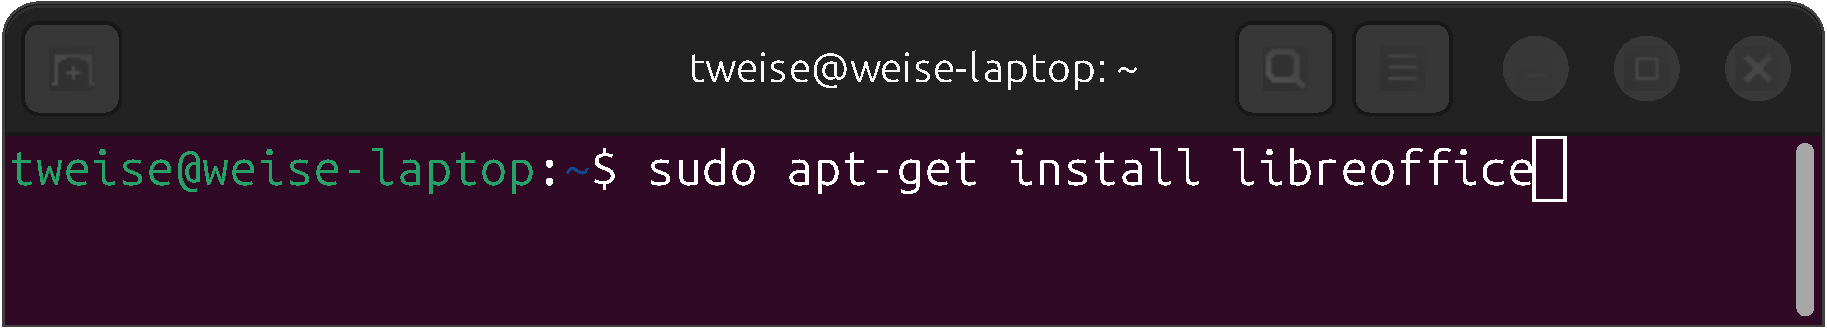
\includegraphics[width=0.7\linewidth]{\currentDir/installingLibreOfficeUbuntu7aptGet}}%
%
\floatRowSep%
%
\subfloat[][%
This requires \pgls{sudo} privileges, so we need to enter the super user password.%
\label{fig:installingLibreOfficeUbuntu8pw}%
]{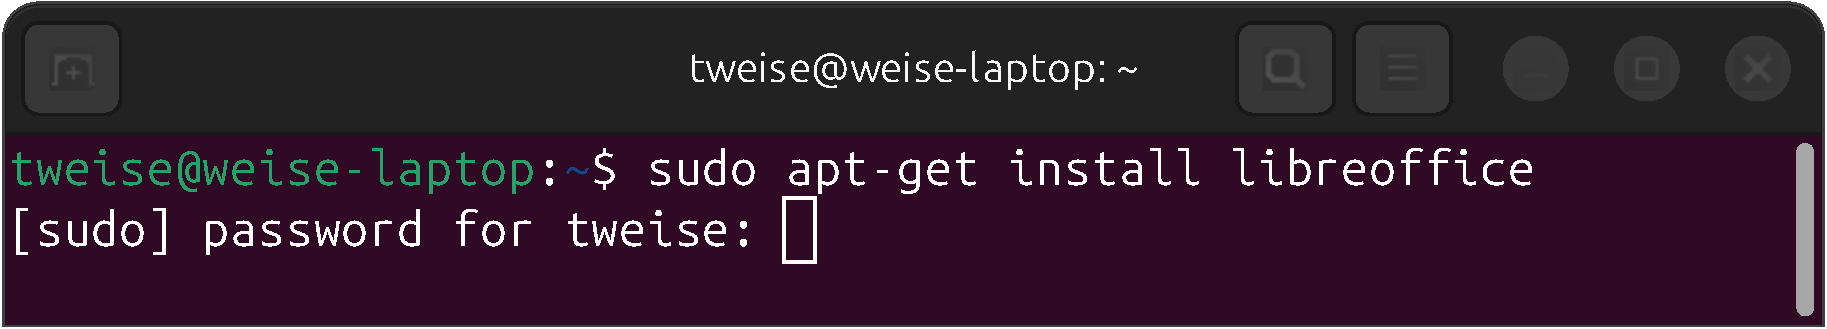
\includegraphics[width=0.7\linewidth]{\currentDir/installingLibreOfficeUbuntu8pw}}%
%
\floatRowSep%
%
\subfloat[][%
Now \libreoffice\ could be installed. %
On my system, it is already installed. %
So nothing happens.%
\label{fig:installingLibreOfficeUbuntu9already}%
]{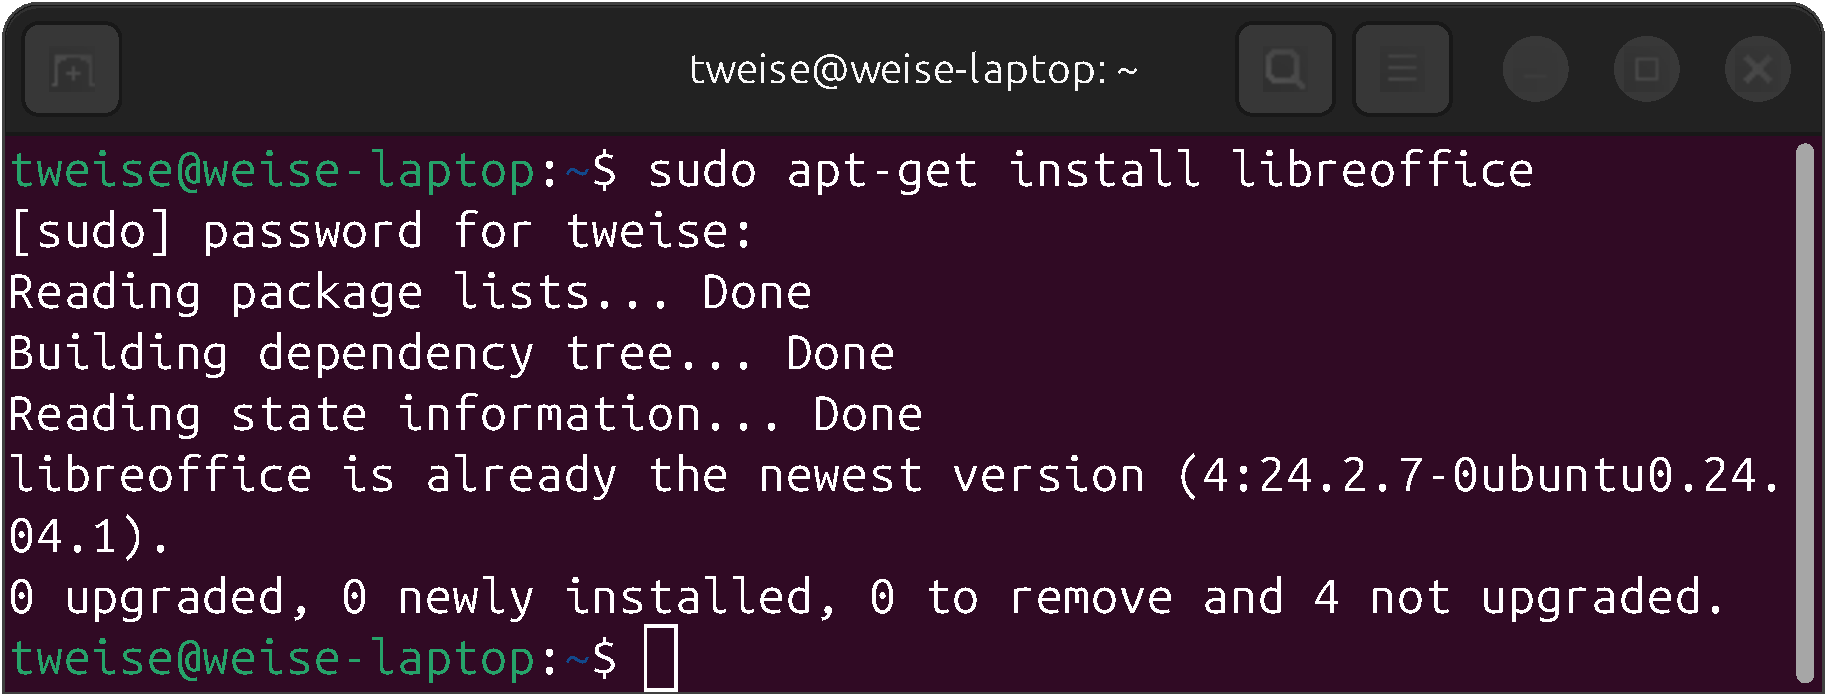
\includegraphics[width=0.7\linewidth]{\currentDir/installingLibreOfficeUbuntu9already}}%
%
\caption{Installing \libreoffice\ under \ubuntu.}%
\label{fig:installingLibreOfficeUbuntuC}%
\end{figure}%
%
If you are a user of \ubuntu\ \linux, then \libreoffice\ and, hence, \libreofficeBase, come already pre-installed on your machine.
You do not actually need to do anything.

To confirm that \libreoffice\ is indeed installed, we open a \pgls{terminal} via with \ubuntuTerminal.
We type \bashil{libreoffice --version} and hit~\keys{\return}.
On my system, the result in \cref{fig:installingLibreOfficeUbuntu1checkVersion} shows that \libreoffice~24.2.7.2 is installed.

We can also start \libreofficeBase\ directly from the \pgls{terminal} by typing \bashil{libreoffice --base} and hitting~\keys{\return}, as show in \cref{fig:installingLibreOfficeUbuntu2runFromTerminal}.
Alternatively, we can open the dash by hitting~\keys{\OSwin}, type \textil{libreoffice}, and then clicking on the symbol for \libreofficeBase, as illustrated in \cref{fig:installingLibreOfficeUbuntu4runFromDash}.
If you do not want to use a hotkey to open the dash, you can also click on the little \ubuntu\ symbol at the bottom-left corner of the screen~(see \cref{fig:installingLibreOfficeUbuntu3openDash}).
Regardless of whether you opened \libreofficeBase\ via a terminal or the dash, the startup screen given in \cref{fig:installingLibreOfficeUbuntu5startupScreen} will appears.
Then, the initial form of \libreofficeBase\ is displayed as shown in \cref{fig:installingLibreOfficeUbuntu6startupForm}.
We are done for now and close the program.%
%
\begin{sloppypar}%
In the unlikely case that \libreoffice\ was not installed on your system, the above will obviously not work.
However, \cref{fig:installingLibreOfficeUbuntu7aptGet} shows that we can easily install it by typing \bashil{sudo apt-get install libreoffice} into a terminal window that we opened with \ubuntuTerminal\ and hit~\keys{\return}.
This requires \pgls{sudo} privileges, so we need to enter the super user password in \cref{fig:installingLibreOfficeUbuntu8pw}.
Now you would probably be told how much data will need to be downloaded, then asked whether you are OK with that, and then \libreoffice\ would be installed.
Since it is already installed on my system, nothing happens. as shown in \cref{fig:installingLibreOfficeUbuntu9already}.%
\end{sloppypar}%
%
The gist is that \libreoffice\ is usally already installed on \ubuntu\ \linux\ or if not, can easily be installed.%
%
\FloatBarrier%
\endhsection%
%
